\documentclass[landscape, oneside, a4paper, cs4size]{book}

\def\marginset#1#2{                      % 页边设置 \marginset{left}{top}
\setlength{\oddsidemargin}{#1}         % 左边(书内侧)装订预留空白距离
\iffalse                   % 如果考虑左侧(书内侧)的边注区则改为\iftrue
\reversemarginpar
\addtolength{\oddsidemargin}{\marginparsep}
\addtolength{\oddsidemargin}{\marginparwidth}
\fi
\setlength{\evensidemargin}{0mm}       % 置0
\iffalse                   % 如果考虑右侧(书外侧)的边注区则改为\iftrue
\addtolength{\evensidemargin}{\marginparsep}
\addtolength{\evensidemargin}{\marginparwidth}
\fi
% \paperwidth = h + \oddsidemargin+\textwidth+\evensidemargin + h
\setlength{\hoffset}{\paperwidth}
\addtolength{\hoffset}{-\oddsidemargin}
\addtolength{\hoffset}{-\textwidth}
\addtolength{\hoffset}{-\evensidemargin}
\setlength{\hoffset}{0.5\hoffset}
\addtolength{\hoffset}{-1in}           % h = \hoffset + 1in
%\setlength{\voffset}{-1in}             % 0 = \voffset + 1in
\setlength{\topmargin}{\paperheight}
\addtolength{\topmargin}{-\headheight}
\addtolength{\topmargin}{-\headsep}
\addtolength{\topmargin}{-\textheight}
\addtolength{\topmargin}{-\footskip}
\addtolength{\topmargin}{#2}           % 上边预留装订空白距离
\setlength{\topmargin}{0.5\topmargin}
}
% 调整页边空白使内容居中,两参数分别为纸的左边和上边预留装订空白距离
\marginset{125mm}{200mm}


%\usepackage{ctex}
\usepackage{bm}
%\usepackage[fleqn]{amsmath}
\usepackage{harpoon}
\usepackage{fontspec}
\usepackage{listings}
\usepackage[left=1cm,right=1cm,top=1cm,bottom=1cm,columnsep=1cm,dvipdfm]{geometry}
\usepackage{setspace}
\usepackage{bm}
\usepackage{cmap}
\usepackage{cite}
\usepackage{float}
\usepackage{xeCJK}
\usepackage{amsthm}
\usepackage{amsmath}
\usepackage{amssymb}
\usepackage{multirow}
\usepackage{multicol}
\usepackage{setspace}
\usepackage{enumerate}
\usepackage{indentfirst}
\usepackage{adjmulticol}
\usepackage{titlesec}
\usepackage[table]{xcolor}
\usepackage{booktabs}
\usepackage[cache=false]{minted}
\usepackage{pdfpages}
\allowdisplaybreaks
%\setlength{\parindent}{0em}
%\setlength{\mathindent}{0pt}
\lstset{breaklines}
\let\cleardoublepage\relax
\titleformat{\chapter}{\normalfont\large\bfseries}{第\,\thechapter\,章}{10pt}{\large}
\titleformat{\section}{\normalfont\normalsize\bfseries}{\thesection}{1em}{}
\titleformat{\subsection}{\normalfont\small\bfseries}{\thesubsection}{1em}{}
\titleformat{\subsubsection}{\normalfont\footnotesize\bfseries}{\thesubsubsection}{1em}{}
\titlespacing*{\chapter} {0pt}{0pt}{0pt}
\titlespacing*{\section} {0pt}{0pt}{0pt}
\titlespacing*{\subsection} {0pt}{-1pt}{-1pt}
\titlespacing*{\subsubsection}{0pt}{-1pt}{-1pt}
\newfontfamily\Courier{Courier New}

\renewcommand{\theFancyVerbLine}{\rmfamily\scriptsize\arabic{FancyVerbLine}}
\newcommand{\cppcode}[1]{
    \inputminted[mathescape,
    			 tabsize=2,
    			 linenos,
    			 %frame=single,
    			 framesep=2mm,
    			 breakaftergroup=true,
    			 breakautoindent=true,
    			 breakbytoken=true,
    			 breaklines=true,
    			 fontsize=\small
    ]{cpp}{source/#1}
}
\newcommand{\javacode}[1]{
    \inputminted[mathescape,
    			 tabsize=2,
    			 linenos,
    			 %frame=single,
    			 framesep=2mm,
    			 breakaftergroup=true,
    			 breakautoindent=true,
    			 breakbytoken=true,
    			 breaklines=true,
    			 fontsize=\small
    ]{java}{source/#1}
}
\newcommand{\vimcode}[1]{
    \inputminted[mathescape,
    			 tabsize=2,
    			 linenos,
    			 %frame=single,
    			 framesep=2mm,
    			 breakaftergroup=true,
    			 breakautoindent=true,
    			 breakbytoken=true,
    			 breaklines=true,
    			 fontsize=\small
    ]{vim}{source/#1}
}
\begin{document}
	\title{\textbf{\LARGE{Standard Code Library}}}
	\author{Shanghai Jiao Tong University, Reshiram}
	\date{October, 2016}
	%\maketitle
	\begin{multicols}{2}\small
	\begin{spacing}{0.72}
	\tableofcontents
	\chapter{计算几何}
		\section{二维几何基础}
		\cppcode{Geometry-Algorithm/Basic2D.cpp}
		\section{快速凸包}
		\cppcode{Geometry-Algorithm/Convex-Hull.cpp}
		\section{半平面交}
		\cppcode{Geometry-Algorithm/Half-Plane-Intersection.cpp}
		\section{三角形的心}
		\cppcode{Geometry-Algorithm/Triangle-Core.cpp}
		\section{圆与多边形面积交}
		\cppcode{Geometry-Algorithm/Circle-Polygon-Intersection.cpp}
		\section{圆并求面积}
		\noindent \textbf{注意事项:}复杂度$\mathcal{O}(n^2\log n)$
		\cppcode{Geometry-Algorithm/Circle-Union.cpp}
		%\section{最近点对}
		\section{最小覆盖圆}
		\cppcode{Geometry-Algorithm/Minimum-Coverage-Circle.cpp}
		%\section{最小覆盖球}
		%\cppcode{Geometry-Algorithm/Minimum-Coverage-Ball.cpp}
		\section{三维几何基础}
		\cppcode{Geometry-Algorithm/Basic3D.cpp}
		\section{三维凸包}
		\cppcode{Geometry-Algorithm/Convex-Hull-3D.cpp}
		\section{三维绕轴旋转}
		\noindent \textbf{注意事项:}以右手拇指为向量方向,逆时针绕轴(剩下四根手指方向)旋转$\theta$角的右乘矩阵。
		\cppcode{Geometry-Algorithm/Rotate-3D.cpp}
		%\section{Delaunay三角剖分}
		%\cppcode{Geometry-Algorithm/Delaunay-Decomposition.cpp}
		%\section{求四点外接球}
	\chapter{图论}
		\section{点双连通分量}
		\cppcode{Graph-Algorithm/Double-Connected-Component.cpp}
		%\section{Hungary求最大匹配}
		%\cppcode{Graph-Algorithm/Maximum-Matching-Hungary.cpp}
		\section{Hopcoft-Karp求最大匹配}
		\cppcode{Graph-Algorithm/Maximum-Matching-Hopcroft-Karp.cpp}
		\section{KM带权匹配}
		\noindent \textbf{注意事项:}最小权完美匹配,复杂度为$\mathcal{O}(|V|^3)$。
		\cppcode{Graph-Algorithm/Maximum-Weight-Matching.cpp}
		\section{稀疏图最大流}
		\noindent \textbf{注意事项:}适用于比较稀疏的一般图。
		\cppcode{Graph-Algorithm/Maximum-Flow-ISAP.cpp}
		\section{稠密图最大流}
		\noindent \textbf{注意事项:}适用于二分图以及一些比较稠密的、增广路径比较短的图。
		\cppcode{Graph-Algorithm/Maximum-Flow-Dinic.cpp}
		%\section{稀疏图费用流}
		%\cppcode{Graph-Algorithm/Minimum-Cost-Maxflow-SPFA.cpp}
		\section{稠密图费用流}
		\cppcode{Graph-Algorithm/Minimum-Cost-Maxflow-ZKW.cpp}
		\section{2-SAT问题}
		\cppcode{Graph-Algorithm/Two-Satisfiability.cpp}
		\section{有根树的同构}
		\cppcode{Graph-Algorithm/Rooted-Tree-Isomorphism.cpp}
		\section{Dominator Tree}
		\cppcode{Graph-Algorithm/Dominator-Tree.cpp}
		%\section{哈密尔顿回路(ORE 性质的图)}
		%\cppcode{Graph-Algorithm/Hamiltonian-Circuit-Ore.cpp}
		\section{无向图最小割}
		\cppcode{Graph-Algorithm/Minimum-Cut-Stoer-Wagner.cpp}
		%\section{弦图判定}
		%\cppcode{Graph-Algorithm/Chord-Graph-Judgement.cpp}
		%\section{弦图求最大团}
		%\cppcode{Graph-Algorithm/Chord-Graph-Group-Counter.cpp}
		\section{最大团搜索}
		\cppcode{Graph-Algorithm/Maximum-Clique-Search.cpp}
		\section{极大团计数}
		\cppcode{Graph-Algorithm/Maximum-Clique-Count.cpp}
		\section{最小树形图}
		\cppcode{Graph-Algorithm/Chu-Liu-Algorithm.cpp}
		\section{带花树}
		\cppcode{Graph-Algorithm/Maximum-Matching-Blossom.cpp}
		%\section{度限制生成树}
		%\cppcode{Graph-Algorithm/Minimum-Spanning-Tree-With-Degree-Limit.cpp}
	\chapter{数论及代数}
		%\section{快速求逆}
		%\cppcode{Mathematical-Algorithm/Quick-Reverse.cpp}
		\section{魔幻多项式}
            \begin{spacing}{0.5}
    			\subsection*{快速傅里叶变换}
    			\noindent \textbf{注意事项:}请实现复数类Complex,并注意快速傅里叶变换精度较差,建议使用快速数论变换。
            \end{spacing}
			\cppcode{Mathematical-Algorithm/Fast-Fourier-Transform.cpp}
			\subsection*{光速数论变换}
            \begin{spacing}{0.5}
    			\noindent \textbf{注意事项:}$\mathrm{MOD}$应该为一个特殊的质数$2^n + 1$且$n$应该要足够大,$\mathrm{PRT}$为这个质数的原根。
            \end{spacing}
			\cppcode{Mathematical-Algorithm/Number-Theory-Transform.cpp}
			\subsection*{牛顿迭代法}
            \begin{spacing}{0.5}
    			\noindent \textbf{问题描述:}给出多项式$G(x)$,求解多项式$F(x)$满足: $\displaystyle G(F(x)) \equiv 0 \pmod {x^n}$
    			答案只需要精确到$F(x) \bmod {x^n}$即可。\par
    			\noindent \textbf{实现原理:}考虑倍增,假设有:
    			\[G(F_t(x)) \equiv 0 \pmod{x^t}\]
    			对$G(F_{t + 1}(x))$在模$x^{2t}$意义下进行Taylor展开:
    			\[G(F_{t + 1}(x)) \equiv G(F_t(x)) + \dfrac{G'(F_t(x))}{1!}(F_{t + 1}(x) - F_t(x)) \pmod{x^{2t}}\]
    			那么就有:$\displaystyle F_{t + 1}(x) \equiv F_t(x) - \dfrac{G(F_t(x))}{G'(F_t(x))} \pmod{x^{2t}}$\par
    			\noindent \textbf{注意事项:}$G(F(x))$的常数项系数必然为0,这个可以作为求解的初始条件;
            \end{spacing}
			\subsection*{多项式求逆}
            \begin{spacing}{0.5}
    			\noindent \textbf{原理:}令$G(x) = x * A - 1$(其中$A$是一个多项式系数),根据牛顿迭代法有:
    			\begin{displaymath}
    				F_{t + 1}(x) \equiv F_t(x) - \dfrac{F_t(x) * A(x) - 1}{A(x)} \equiv 2F_t(x) - F_t(x)^2 * A(x)\pmod{x^{2t}}
    			\end{displaymath}
    			\noindent \textbf{注意事项:}
    			\begin{enumerate}
    				\item $F(x)$的常数项系数必然不为0,否则没有逆元;
    				\item 复杂度是$O(n \log n)$但是常数比较大($10^5$大概需要0.3秒左右);
    				\item 传入的两个数组必须不同,但传入的次数界没有必要是2的次幂;
    			\end{enumerate}
            \end{spacing}
			\cppcode{Mathematical-Algorithm/Polynomial-Inverse.cpp}
			\subsection*{多项式取指数和对数}
            \begin{spacing}{0.5}
    			\noindent \textbf{作用:}给出一个多项式$A(x)$,求一个多项式$F(x)$满足$e^A(x) - F(x) \equiv 0 \pmod{x^n}$。\par
    			\noindent \textbf{原理:}令$G(x) = \ln x - A$(其中$A$是一个多项式系数),根据牛顿迭代法有:
    			\[F_{t + 1}(x) \equiv F_t(x) - F_t(x)(\ln {F_t(x)} - A(x)) \pmod{x^{2t}}\]
    			求$\ln {F_t(x)}$可以用先求导再积分的办法,即:$\displaystyle \ln A(x) = \int \dfrac{F'(x)}{F(x)}~\mathrm{d}x$
    			多项式的求导和积分可以在$O(n)$的时间内完成,因此总复杂度为$O(n \log n)$。\par
    			\noindent \textbf{应用:}加速多项式快速幂。\par
    			\noindent \textbf{注意事项:}
    			\begin{enumerate}
    				\item 进行$\log$的多项式必须保证常数项系数为1,否则必须要先求出$\log a[0]$是多少;
    				\item 传入的两个数组必须不同,但传入的次数界没有必要是2的次幂;
    				\item 常数比较大,$10^5$的数据求指数和对数分别需要0.37s和0.85s左右的时间,注意这里\Courier{memset}几乎不占用时。
    			\end{enumerate}
            \end{spacing}
			\cppcode{Mathematical-Algorithm/Polynomial-ExpAndLn.cpp}
			\subsection*{多项式除法}
            \begin{spacing}{0.5}
    			\noindent \textbf{作用:}给出两个多项式$A(x)$和$B(x)$,求两个多项式$D(x)$和$R(x)$满足:
    			\[A(x) \equiv D(x)B(x) + R(x) \pmod{x^n}\]
    			\noindent \textbf{注意事项:}
    			\begin{enumerate}
    				\item 常数比较大概为6倍FFT的时间,即大约$10^5$的数据0.07s左右;
    				\item 传入两个多项式的次数界,没有必要是2的次幂,但是要保证除数多项式不为0。
    			\end{enumerate}
            \end{spacing}
			\cppcode{Mathematical-Algorithm/Polynomial-Division.cpp}
		\section{线性递推数列求第$n$项}
		\cppcode{Mathematical-Algorithm/Linear-Recurrence.cpp}
		\section{线性规划}
		\noindent \textbf{注意事项:}使用单纯形法求解:
		\[max\{c_{1 \times m} \cdot x_{m \times 1} \ | \ x_{m \times 1} \geq 0_{m \times 1}, a_{n \times m} \cdot x_{m \times 1} \leq b_{n \times 1}\}\]
		\cppcode{Mathematical-Algorithm/Simplex.cpp}
		%\section{Schreier-Sims}
		\section{中国剩余定理}
		\noindent \textbf{注意事项:}$p_i$无需两两互质
		\cppcode{Mathematical-Algorithm/Chinese-Remainder-Theorem.cpp}
		\section{直线下整点个数}
		\noindent \textbf{注意事项:}返回结果为:$\displaystyle \sum_{0 \leq i < n} \lfloor \frac{a + b \cdot i}{m} \rfloor$
		即直线下整点个数。
		\cppcode{Mathematical-Algorithm/Lattice-Counter.cpp}
		\section{闪电素数判定}
		\cppcode{Mathematical-Algorithm/Miller-Rabin.cpp}
		\section{闪电质因数分解}
		\cppcode{Mathematical-Algorithm/Pollard-Rho.cpp}
		\section{⾃适应⾟普森}
		\cppcode{Mathematical-Algorithm/Self-Adjusting-Simpson.cpp}
		\section{二次剩余}
		\cppcode{Mathematical-Algorithm/Quad-Remainder.cpp}
		\section{Pell 方程}
		\cppcode{Mathematical-Algorithm/Pell.cpp}
		\section{原根相关}
		\begin{enumerate}
			\item 模$m$有原根的充要条件:$m = 2, 4, p^a, 2p^a$,其中$p$是奇素数;
			\item 求任意数$p$原根的方法:对$\phi(p)$因式分解,即$\phi(p) = p_1^{r_1}p_2^{r_2}\cdots p_k^{r_k}$,若恒成立:
			\[g^{\frac{p - 1}{g}} \neq 1 \pmod{p}\]
			那么$g$就是$p$的原根。
			\item 若模$m$有原根,那么它一共有$\phi(\phi(m))$个原根。
		\end{enumerate}
	\chapter{字符串}
		\section{广义后缀自动机}
		\noindent \textbf{注意事项:}空间是插入字符串总长度的2倍并请注意字符集大小。
		\cppcode{String-Algorithm/Generalized-Suffix-Automaton.cpp}
		\section{后缀数组}
		\noindent \textbf{注意事项:}$\mathcal{O}(n\log n)$倍增构造。
		\cppcode{String-Algorithm/Suffix-Array.cpp}
		\section{回文自动机}
		\noindent \textbf{注意事项:}请注意字符集大小。
		\cppcode{String-Algorithm/Palindromic-Automaton.cpp}
		\section{Manacher}
		\noindent \textbf{注意事项:}1-based算法,请注意下标。
		\cppcode{String-Algorithm/Manacher.cpp}
		\section{循环串的最小表示}
		\noindent \textbf{注意事项:}0-Based算法,请注意下标。
		\cppcode{String-Algorithm/Minimum-Representation.cpp}
		\section{后缀树}
		\noindent \textbf{注意事项:}
		\begin{enumerate}
			\item \indent 边上的字符区间是左闭右开区间;
			\item \indent 如果要建立关于多个串的后缀树,请用不同的分隔符,并且对于每个叶子结点,去掉和它父亲的连边上出现的第一个分隔符之后的所有字符;
		\end{enumerate}
		\cppcode{String-Algorithm/Suffix-Tree.cpp}
	\chapter{数据结构}
		\section{树链剖分}
		\subsection*{点操作版本}
		\cppcode{Data-Structure/Heavy-Light-Decomposition-Point.cpp}
		\subsection*{边操作版本}
		\cppcode{Data-Structure/Heavy-Light-Decomposition-Chain.cpp}
		\section{Link Cut Tree}
		\cppcode{Data-Structure/Link-Cut-Tree.cpp}
		\section{可持久化平衡树}
		\cppcode{Data-Structure/Persistent-Treap.cpp}
		\section{可持久化左偏树}
		\cppcode{Data-Structure/Leftist-Heap.cpp}
		%\section{Splay Tree}
		%\subsection*{区间操作版本}
		%\cppcode{Data-Structure/Splay-Interval.cpp}
		%\subsection*{序列操作版本}
		%\cppcode{Data-Structure/Splay-Sequence.cpp}
		\section{k-d Tree}
		\cppcode{Data-Structure/K-d-Tree.cpp}
	\chapter{杂项算法}
		\section{Dancing Links}
		\cppcode{Incidental-Algorithm/Dancing-Links.cpp}
		\section{日期公式}
		\cppcode{Incidental-Algorithm/Date-Lemma.cpp}
		%\section{环状最长公共子序列}
		%\cppcode{Incidental-Algorithm/Cycle-Longest.cpp}
		\section{经纬度球面距离}
		\cppcode{Incidental-Algorithm/Ball-Distance.cpp}
		%\section{长方体表面两点最短距离}
		%\cppcode{Incidental-Algorithm/Minimum-Distance-Cube.cpp}
	\chapter{其他}
		\section{Java Hints}
		\javacode{Hint/Java-Hints.java}
		\section{vimrc}
		\vimcode{Hint/vimrc}
        \begin{spacing}{0.50}
		\section{常用结论}\footnotesize
        \begin{spacing}{0.5}
			\subsection*{上下界网络流}
			$B(u,v)$表示边$(u,v)$流量的下界,$C(u,v)$表示边$(u,v)$流量的上界,$F(u,v)$表示边$(u,v)$的流量。
			设$G(u,v) = F(u,v) - B(u,v)$,显然有:$\displaystyle 0 \leq G(u,v) \leq C(u,v)-B(u,v)$
			\subsubsection*{无源汇的上下界可行流}
			建立超级源点$S^*$和超级汇点$T^*$,对于原图每条边$(u,v)$在新网络中连如下三条边:$S^* \rightarrow v$,容量为$B(u,v)$;$u \rightarrow T^*$,容量为$B(u,v)$;$u \rightarrow v$,容量为$C(u,v) - B(u,v)$。最后求新网络的最大流,判断从超级源点$S^*$出发的边是否都满流即可,边$(u,v)$的最终解中的实际流量为$G(u,v)+B(u,v)$。
			\subsubsection*{有源汇的上下界可行流}
			从汇点$T$到源点$S$连一条上界为$\infty$,下界为$0$的边。按照\textbf{无源汇的上下界可行流}一样做即可,流量即为$T \rightarrow S$边上的流量。
			\subsubsection*{有源汇的上下界最大流}
			\begin{enumerate}
				\item 在\textbf{有源汇的上下界可行流}中,从汇点$T$到源点$S$的边改为连一条上界为$\infty$,下届为$x$的边。$x$满足二分性质,找到最大的$x$使得新网络存在\textbf{无源汇的上下界可行流}即为原图的最大流。
				\item 从汇点$T$到源点$S$连一条上界为$\infty$,下界为$0$的边,变成无源汇的网络。按照\textbf{无源汇的上下界可行流}的方法,建立超级源点$S^*$和超级汇点$T^*$,求一遍$S^* \rightarrow T^*$的最大流,再将从汇点$T$到源点$S$的这条边拆掉,求一次$S \rightarrow T$的最大流即可。
			\end{enumerate}
			\subsubsection*{有源汇的上下界最小流}
			\begin{enumerate}
				\item 在\textbf{有源汇的上下界可行流}中,从汇点$T$到源点$S$的边改为连一条上界为$x$,下界为$0$的边。$x$满足二分性质,找到最小的$x$使得新网络存在\textbf{无源汇的上下界可行流}即为原图的最小流。
				\item 按照\textbf{无源汇的上下界可行流}的方法,建立超级源点$S^*$与超级汇点$T^*$,求一遍$S^* \rightarrow T^*$的最大流,但是注意这一次不加上汇点$T$到源点$S$的这条边,即不使之改为无源汇的网络去求解。求完后,再加上那条汇点$T$到源点$S$上界$\infty$的边。因为这条边下界为$0$,所以$S^*$,$T^*$无影响,再直接求一次$S^* \rightarrow T^*$的最大流。若超级源点$S^*$出发的边全部满流,则$T \rightarrow S$边上的流量即为原图的最小流,否则无解。
			\end{enumerate}
			\subsection*{上下界费用流}
			\noindent \textbf{来源:BZOJ 3876}
			\noindent 设汇$t$,源$s$,超级源$S$,超级汇$T$,本质是每条边的下界为1,上界为$MAX$,跑一遍有源汇的上下界最小费用最小流。(因为上界无穷大,所以只要满足所有下界的最小费用最小流)
			\begin{enumerate}
				\item 对每个点$x$:从$x$到$t$连一条费用为0,流量为MAX的边,表示可以任意停止当前的剧情(接下来的剧情从更优的路径去走,画个样例就知道了)
				\item 对于每一条边权为$z$的边$x \rightarrow y$:
				\begin{itemize}
					\item 从$S$到$y$连一条流量为1,费用为$z$的边,代表这条边至少要被走一次。
					\item 从$x$到$y$连一条流量为$MAX$,费用为$z$的边,代表这条边除了至少走的一次之外还可以随便走。
					\item 从$x$到$T$连一条流量为1,费用为0的边。(注意是每一条$x->y$的边都连,或者你可以记下$x$的出边数$K_x$,连一次流量为$K_x$,费用为0的边)。
				\end{itemize}
			\end{enumerate}
			建完图后从S到T跑一遍费用流,即可。(当前跑出来的就是满足上下界的最小费用最小流了)
			\subsection*{弦图相关}
			\begin{enumerate}
				\item[1.] 团数 $\leq$ 色数 , 弦图团数 = 色数
				\item[2.] 设 $next(v)$ 表示 $N(v)$ 中最前的点 .
				令 w* 表示所有满足 $A \in B$ 的 w 中最后的一个点 ,
				判断 $v \cup N(v)$ 是否为极大团 ,
				只需判断是否存在一个 w,
				满足 $Next(w)=v$ 且 $|N(v)| + 1 \leq |N(w)|$ 即可 .
				\item[3.] 最小染色 : 完美消除序列从后往前依次给每个点染色 ,
				给每个点染上可以染的最小的颜色
				\item[4.] 最大独立集 : 完美消除序列从前往后能选就选
				\item[5.] 弦图最大独立集数 $=$ 最小团覆盖数 ,
				最小团覆盖 :
				设最大独立集为 $\{p_1,p_2, \dots ,p_t\}$,
				则 $\{p_1\cup N(p_1), \dots , p_t \cup N(p_t)\}$
				为最小团覆盖
			\end{enumerate}
			\subsection*{Bernoulli数}
				\begin{enumerate}
	\item 初始化:$B_0(n) = 1$
	\item 递推公式:
	\[B_m(n) = n^m - \sum_{k = 0}^{m - 1}\binom{m}{k} \frac{B_k(n)}{m - k + 1}\]
	\item 应用:
	\[\sum_{k = 1}^{n} k^m = \frac{1}{m + 1}\sum_{k = 0}^{m}\binom{m + 1}{k}n^{m + 1 - k}\]
\end{enumerate}


        \end{spacing}
		\section{常见错误}\footnotesize
		\begin{enumerate}
			\item 数组或者变量类型开错,例如将double开成int;
			\item 函数忘记返回返回值;
			\item 初始化数组没有初始化完全;
			\item 对空间限制判断不足导致MLE;
		\end{enumerate}
		\section{博弈游戏}\footnotesize
		\subsection{巴什博奕}
	\begin{enumerate}\setlength{\itemsep}{-\itemsep}
		\item 
			只有一堆n个物品,两个人轮流从这堆物品中取物,规定每次至少取一个,最多取m个。最后取光者得胜。
		\item
			显然,如果$n=m+1$,那么由于一次最多只能取$m$个,所以,无论先取者拿走多少个,
			后取者都能够一次拿走剩余的物品,后者取胜。因此我们发现了如何取胜的法则:如果
			$n=(m+1)r+s$,(r为任意自然数,$s \leq m$),那么先取者要拿走$s$个物品,
			如果后取者拿走$k(k \leq m)$个,那么先取者再拿走$m+1-k$个,结果剩下$(m+1)(r-1)$
			个,以后保持这样的取法,那么先取者肯定获胜。总之,要保持给对手留下$(m+1)$的倍数,
			就能最后获胜。
	\end{enumerate}
\subsection{威佐夫博弈}
	\begin{enumerate}\setlength{\itemsep}{-\itemsep}
		\item 
			有两堆各若干个物品,两个人轮流从某一堆或同时从两堆中取同样多的物品,规定每次至少取
			一个,多者不限,最后取光者得胜。
		\item
			判断一个局势$(a, b)$为奇异局势(必败态)的方法:
			$$a_k =[k (1+\sqrt{5})/2],b_k= a_k + k$$
	\end{enumerate}
\subsection{阶梯博奕}
	\begin{enumerate}\setlength{\itemsep}{-\itemsep}
		\item
			博弈在一列阶梯上进行,每个阶梯上放着自然数个点,两个人进行阶梯博弈,
			每一步则是将一个阶梯上的若干个点(至少一个)移到前面去,最后没有点
			可以移动的人输。
		\item
			解决方法:把所有奇数阶梯看成N堆石子,做NIM。(把石子从奇数堆移动到偶数
			堆可以理解为拿走石子,就相当于几个奇数堆的石子在做Nim)
	\end{enumerate}
\subsection{图上删边游戏}
	\subsubsection{链的删边游戏}
		\begin{enumerate}\setlength{\itemsep}{-\itemsep}
			\item
				游戏规则:对于一条链,其中一个端点是根,两人轮流删边,脱离根的部分也算被删去,最后没边可删的人输。
			\item
				做法:$sg[i] = n - dist(i) - 1$(其中$n$表示总点数,$dist(i)$表示离根的距离)
		\end{enumerate}
	\subsubsection{树的删边游戏}
		\begin{enumerate}\setlength{\itemsep}{-\itemsep}
			\item
				游戏规则:对于一棵有根树,两人轮流删边,脱离根的部分也算被删去,没边可删的人输。
			\item
				做法:叶子结点的$sg=0$,其他节点的$sg$等于儿子结点的$sg+1$的异或和。
		\end{enumerate}
	\subsubsection{局部连通图的删边游戏}
		\begin{enumerate}\setlength{\itemsep}{-\itemsep}
			\item
				游戏规则:在一个局部连通图上,两人轮流删边,脱离根的部分也算被删去,没边可删的人输。
				局部连通图的构图规则是,在一棵基础树上加边得到,所有形成的环保证不共用边,且只与基础树有一个公共点。
			\item
				做法:去掉所有的偶环,将所有的奇环变为长度为1的链,然后做树的删边游戏。
		\end{enumerate}

		\section{常用数学公式}\footnotesize
		\begin{spacing}{0.1}
\subsection*{求和公式}
	\begin{enumerate}
		\item $\sum_{k=1}^{n}(2k-1)^2 = \frac{n(4n^2-1)}{3}	$
		\item $\sum_{k=1}^{n}k^3 = [\frac{n(n+1)}{2}]^2	$
		\item $\sum_{k=1}^{n}(2k-1)^3 = n^2(2n^2-1)	$
		\item $\sum_{k=1}^{n}k^4 = \frac{n(n+1)(2n+1)(3n^2+3n-1)}{30}  $
		\item $\sum_{k=1}^{n}k^5 = \frac{n^2(n+1)^2(2n^2+2n-1)}{12}	$
		\item $\sum_{k=1}^{n}k(k+1) = \frac{n(n+1)(n+2)}{3}	$
		\item $\sum_{k=1}^{n}k(k+1)(k+2) = \frac{n(n+1)(n+2)(n+3)}{4} $
		\item $\sum_{k=1}^{n}k(k+1)(k+2)(k+3) = \frac{n(n+1)(n+2)(n+3)(n+4)}{5} $
		\item $\displaystyle \frac{1}{(1 - x)^{n + 1}} = \sum_{i = 0}^{n}\binom{i + n}{i}x^i$
		\item $\displaystyle \frac{1}{\sqrt{1 - 4x}} = \sum_{i = 0}^{n}\binom{2i}{i}x^i$
	\end{enumerate}
\subsection*{斐波那契数列}
	\begin{enumerate}
		\item $fib_0=0, fib_1=1, fib_n=fib_{n-1}+fib_{n-2}$
		\item $fib_{n+2} \cdot fib_n-fib_{n+1}^2=(-1)^{n+1}$
		\item $fib_{-n}=(-1)^{n-1}fib_n$
		\item $fib_{n+k}=fib_k \cdot fib_{n+1}+fib_{k-1} \cdot fib_n$
		\item $gcd(fib_m, fib_n)=fib_{gcd(m, n)}$
		\item $fib_m|fib_n^2\Leftrightarrow nfib_n|m$
	\end{enumerate}
\subsection*{错排公式}
	\[D_n = (n-1)(D_{n-2}-D_{n-1})= = n! \cdot (1-\frac{1}{1!}+\frac{1}{2!}-\frac{1}{3!}+\ldots+\frac{(-1)^n}{n!})\]
\subsection*{莫比乌斯函数}
	$$\mu(n) = \begin{cases}
		1 & \text{若}n=1\\
		(-1)^k & \text{若}n\text{无平方数因子,且}n = p_1p_2\dots p_k\\
		0 & \text{若}n\text{有大于}1\text{的平方数因数}
	\end{cases}$$
	$$\sum_{d|n}{\mu(d)} = \begin{cases}
		1 & \text{若}n=1\\
		0 & \text{其他情况}
	\end{cases}$$
	$$g(n) = \sum_{d|n}{f(d)} \Leftrightarrow f(n) = \sum_{d|n}{\mu(d)g(\frac{n}{d})}$$
	$$g(x) = \sum_{n=1}^{[x]}f(\frac{x}{n}) \Leftrightarrow f(x) = \sum_{n=1}^{[x]}{\mu(n)g(\frac{x}{n})}$$
\subsection*{Burnside引理}
	设$G$是一个有限群,作用在集合$X$上。对每个$g$属于$G$,令$X^g$表示$X$中在$g$作用下的不动元素,轨道数(记作$|X/G|$)为$\displaystyle |X/G| = \frac{1}{|G|}\sum_{g \in G}|X^g|.\,$
\subsection*{五边形数定理}
	设$p(n)$是$n$的拆分数,有$\displaystyle p(n) = \sum_{k \in \mathbb{Z} \setminus \{0\}} (-1)^{k - 1} p\left(n - \frac{k(3k - 1)}{2}\right)$
\subsection*{树的计数}
	\begin{enumerate}
		\item 有根树计数:$n+1$个结点的有根树的个数为$\displaystyle a_{n+1} = \frac{\sum_{j=1}^{n}{j \cdot a_j \cdot{S_{n, j}}}}{n}$,其中,$\displaystyle S_{n, j} = \sum_{i=1}^{n/j}{a_{n+1-ij}} = S_{n-j, j} + a_{n+1-j}$
		\item 无根树计数:当$n$为奇数时,$n$个结点的无根树的个数为$a_n-\sum_{i=1}^{n/2}{a_ia_{n-i}}$,当$n$为偶数时,$n$个结点的无根树的个数为$a_n-\sum_{i=1}^{n/2}{a_ia_{n-i}}+\frac{1}{2}a_{\frac{n}{2}}(a_{\frac{n}{2}}+1)$
		\item $n$个结点的完全图的生成树个数为:$\displaystyle n^{n-2}$
		\item 矩阵-树定理:
		图$G$由$n$个结点构成,设$\bm{A}[G]$为图$G$的邻接矩阵、$\bm{D}[G]$为图$G$的度数矩阵,
		则图$G$的不同生成树的个数为$\bm{C}[G] = \bm{D}[G] - \bm{A}[G]$的任意一个$n-1$阶主子式的行列式值。
	\end{enumerate}
\subsection*{欧拉公式}
	平面图的顶点个数、边数和面的个数有如下关系:$\displaystyle V - E + F = C+ 1$\par
	其中,$V$是顶点的数目,$E$是边的数目,$F$是面的数目,$C$是组成图形的连通部分的数目。当图是单连通图的时候,公式简化为:$\displaystyle V - E + F = 2$
\subsection*{皮克定理}
	给定顶点坐标均是整点(或正方形格点)的简单多边形,其面积$A$和内部格点数目$i$、边上格点数目$b$的关系:$A = i + \frac{b}{2} - 1$
\subsection*{牛顿恒等式}
	设$$\prod_{i = 1}^n{(x - x_i)} = a_n + a_{n - 1} x + \dots + a_1 x^{n - 1} + a_0 x^n$$
	$$p_k = \sum_{i = 1}^n{x_i^k}$$
	则$$a_0 p_k + a_1 p_{k - 1} + \cdots + a_{k - 1} p_1 + k a_k = 0$$\par
	特别地,对于$$|\bm{A} - \lambda \bm{E}| = (-1)^n(a_n + a_{n - 1} \lambda + \cdots + a_1 \lambda^{n - 1} + a_0 \lambda^n)$$
	有$$p_k = \mathrm{Tr}(\bm{A}^k)$$
%\section{数论公式}
\section{平面几何公式}
\subsection*{三角形}
\begin{spacing}{0.1}
	\begin{enumerate}
		\item 面积:$\displaystyle S=\frac{a \cdot H_a}{2}=\frac{ab \cdot sinC}{2}=\sqrt{p(p-a)(p-b)(p-c)}\left(\frac{a + b + c}{2}\right)$
		\item 中线:$\displaystyle M_a=\frac{\sqrt{2(b^2+c^2)-a^2}}{2}=\frac{\sqrt{b^2+c^2+2bc \cdot cosA}}{2}$
		\item 角平分线:$\displaystyle T_a=\frac{\sqrt{bc \cdot [(b+c)^2-a^2]}}{b+c}=\frac{2bc}{b+c}cos\frac{A}{2}$
		\item 高线:$\displaystyle H_a=bsinC=csinB=\sqrt{b^2-(\frac{a^2+b^2-c^2}{2a})^2}$
		\item 内切圆半径
			\begin{align*}
				r&=\frac{S}{p}=\frac{arcsin\frac{B}{2} \cdot sin\frac{C}{2}}{sin\frac{B+C}{2}}=4R \cdot sin\frac{A}{2}sin\frac{B}{2}sin\frac{C}{2}\\
				&=\sqrt{\frac{(p-a)(p-b)(p-c)}{p}}=p \cdot tan\frac{A}{2}tan\frac{B}{2}tan\frac{C}{2}
			\end{align*}
		\item 外接圆半径:$\displaystyle R=\frac{abc}{4S}=\frac{a}{2sinA}=\frac{b}{2sinB}=\frac{c}{2sinC}$
	\end{enumerate}
\end{spacing}
\subsection*{四边形}
\begin{spacing}{0.1}
	$D_1, D_2$为对角线,$M$对角线中点连线,$A$为对角线夹角,$p$为半周长
	\begin{enumerate}
		\item $a^2+b^2+c^2+d^2=D_1^2+D_2^2+4M^2$
		\item $S=\frac{1}{2}D_1D_2sinA$
		\item 对于圆内接四边形:$\displaystyle ac+bd=D_1D_2$
		\item 对于圆内接四边形:$\displaystyle S=\sqrt{(p-a)(p-b)(p-c)(p-d)}$
	\end{enumerate}
\end{spacing}
\subsection*{正$n$边形}
\begin{spacing}{0.1}
	$R$为外接圆半径,$r$为内切圆半径
	\begin{enumerate}
		\item 中心角:$\displaystyle A=\frac{2\pi}{n}$
		\item 内角:$\displaystyle C=\frac{n-2}{n}\pi$
		\item 边长:$\displaystyle a=2\sqrt{R^2-r^2}=2R \cdot sin\frac{A}{2}=2r \cdot tan\frac{A}{2}$
		\item 面积:$\displaystyle S=\frac{nar}{2}=nr^2 \cdot tan\frac{A}{2}=\frac{nR^2}{2} \cdot sinA=\frac{na^2}{4 \cdot tan\frac{A}{2}}$
	\end{enumerate}
\end{spacing}
\subsection*{圆}
\begin{spacing}{0.1}
	\begin{enumerate}
		\item 弧长:$\displaystyle l=rA$
		\item 弦长:$\displaystyle a=2\sqrt{2hr-h^2}=2r\cdot sin\frac{A}{2}$
		\item 弓形高:$\displaystyle h=r-\sqrt{r^2-\frac{a^2}{4}}=r(1-cos\frac{A}{2})=\frac{1}{2} \cdot arctan\frac{A}{4}$
		\item 扇形面积:$\displaystyle S_1=\frac{rl}{2}=\frac{r^2A}{2}$
		\item 弓形面积:$\displaystyle S_2=\frac{rl-a(r-h)}{2}=\frac{r^2}{2}(A-sinA)$
	\end{enumerate}
\end{spacing}
\subsection*{棱柱}
\begin{spacing}{0.1}
	\begin{enumerate}
		\item 体积($A$为底面积,$h$为高):$\displaystyle V=Ah$
		\item 侧面积($l$为棱长,$p$为直截面周长):$\displaystyle S=lp$
		\item 全面积:$\displaystyle T=S+2A$
	\end{enumerate}
\end{spacing}
\subsection*{棱锥}
\begin{spacing}{0.1}
	\begin{enumerate}
		\item 体积($A$为底面积,$h$为高):$\displaystyle V=Ah$
		\item 正棱锥侧面积($l$为棱长,$p$为直截面周长):$\displaystyle S=lp$
		\item 正棱锥全面积:$\displaystyle T=S+2A$
	\end{enumerate}
\end{spacing}
\subsection*{棱台}
\begin{spacing}{0.1}
	\begin{enumerate}
		\item 体积($A_1,A_2$为上下底面积,$h$为高):$\displaystyle V=(A_1+A_2+\sqrt{A_1A_2}) \cdot \frac{h}{3}$
		\item 正棱台侧面积($p_1,p_2$为上下底面周长,$l$为斜高):$\displaystyle S=\frac{p_1+p_2}{2}l$
		\item 正棱台全面积:$\displaystyle T=S+A_1+A_2$
	\end{enumerate}
\end{spacing}
\subsection*{圆柱}
\begin{spacing}{0.1}
	\begin{enumerate}
		\item 侧面积:$\displaystyle S=2\pi rh$
		\item 全面积:$\displaystyle T=2\pi r(h+r)$
		\item 体积:$\displaystyle V=\pi r^2h$
	\end{enumerate}
\end{spacing}
\subsection*{圆锥}
\begin{spacing}{0.1}
	\begin{enumerate}
		\item 母线:$\displaystyle l=\sqrt{h^2+r^2}$
		\item 侧面积:$\displaystyle S=\pi rl$
		\item 全面积:$\displaystyle T=\pi r(l+r)$
		\item 体积:$\displaystyle V=\frac{\pi}{3} r^2h$
	\end{enumerate}
\end{spacing}
\subsection*{圆台}
\begin{spacing}{0.1}
	\begin{enumerate}
		\item 母线:$\displaystyle l=\sqrt{h^2+(r_1-r_2)^2}$
		\item 侧面积:$\displaystyle S=\pi(r_1+r_2)l$
		\item 全面积:$\displaystyle T=\pi r_1(l+r_1)+\pi r_2(l+r_2)$
		\item 体积:$\displaystyle V=\frac{\pi}{3}(r_1^2+r_2^2+r_1r_2)h$
	\end{enumerate}
\end{spacing}
\subsection*{球}
\begin{spacing}{0.1}
	\begin{enumerate}
		\item 全面积:$\displaystyle T=4\pi r^2$
		\item 体积:$\displaystyle V=\frac{4}{3}\pi r^3$
	\end{enumerate}
\end{spacing}
\subsection*{球台}
\begin{spacing}{0.1}
	\begin{enumerate}
		\item 侧面积:$\displaystyle S=2\pi rh$
		\item 全面积:$\displaystyle T=\pi(2rh+r_1^2+r_2^2)$
		\item 体积:$\displaystyle V=\frac{\pi h[3(r_1^2+r_2^2)+h^2]}{6}$
	\end{enumerate}
\end{spacing}
\subsection*{球扇形}
\begin{spacing}{0.1}
	\begin{enumerate}
		\item 全面积($h$为球冠高,$r_0$为球冠底面半径):$\displaystyle T=\pi r(2h+r_0)$
		\item 体积:$\displaystyle V=\frac{2}{3}\pi r^2h$
	\end{enumerate}
\end{spacing}
\section{立体几何公式}
\subsection*{球面三角公式}
	设$a, b, c$是边长,$A, B, C$是所对的二面角,
	有余弦定理$$cos a = cos b \cdot cos c + sin b \cdot sin c \cdot cos A$$
	正弦定理$$\frac{sin A}{sin a} = \frac{sin B}{sin b} = \frac{sin C}{sin c}$$
	三角形面积是$A + B + C - \pi$
\subsection*{四面体体积公式}
	$U, V, W, u, v, w$是四面体的$6$条棱,$U, V, W$构成三角形,$(U, u), (V, v), (W, w)$互为对棱,
	则$$V = \frac{\sqrt{(s - 2a)(s - 2b)(s - 2c)(s - 2d)}}{192 uvw}$$
	其中$$\left\{\begin{array}{lll}
			a & = & \sqrt{xYZ}, \\
			b & = & \sqrt{yZX}, \\
			c & = & \sqrt{zXY}, \\
			d & = & \sqrt{xyz}, \\
			s & = & a + b + c + d, \\
			X & = & (w - U + v)(U + v + w), \\
			x & = & (U - v + w)(v - w + U), \\
			Y & = & (u - V + w)(V + w + u), \\
			y & = & (V - w + u)(w - u + V), \\
			Z & = & (v - W + u)(W + u + v), \\
			z & = & (W - u + v)(u - v + W)
		\end{array}\right.$$
\end{spacing}

        \end{spacing}
		%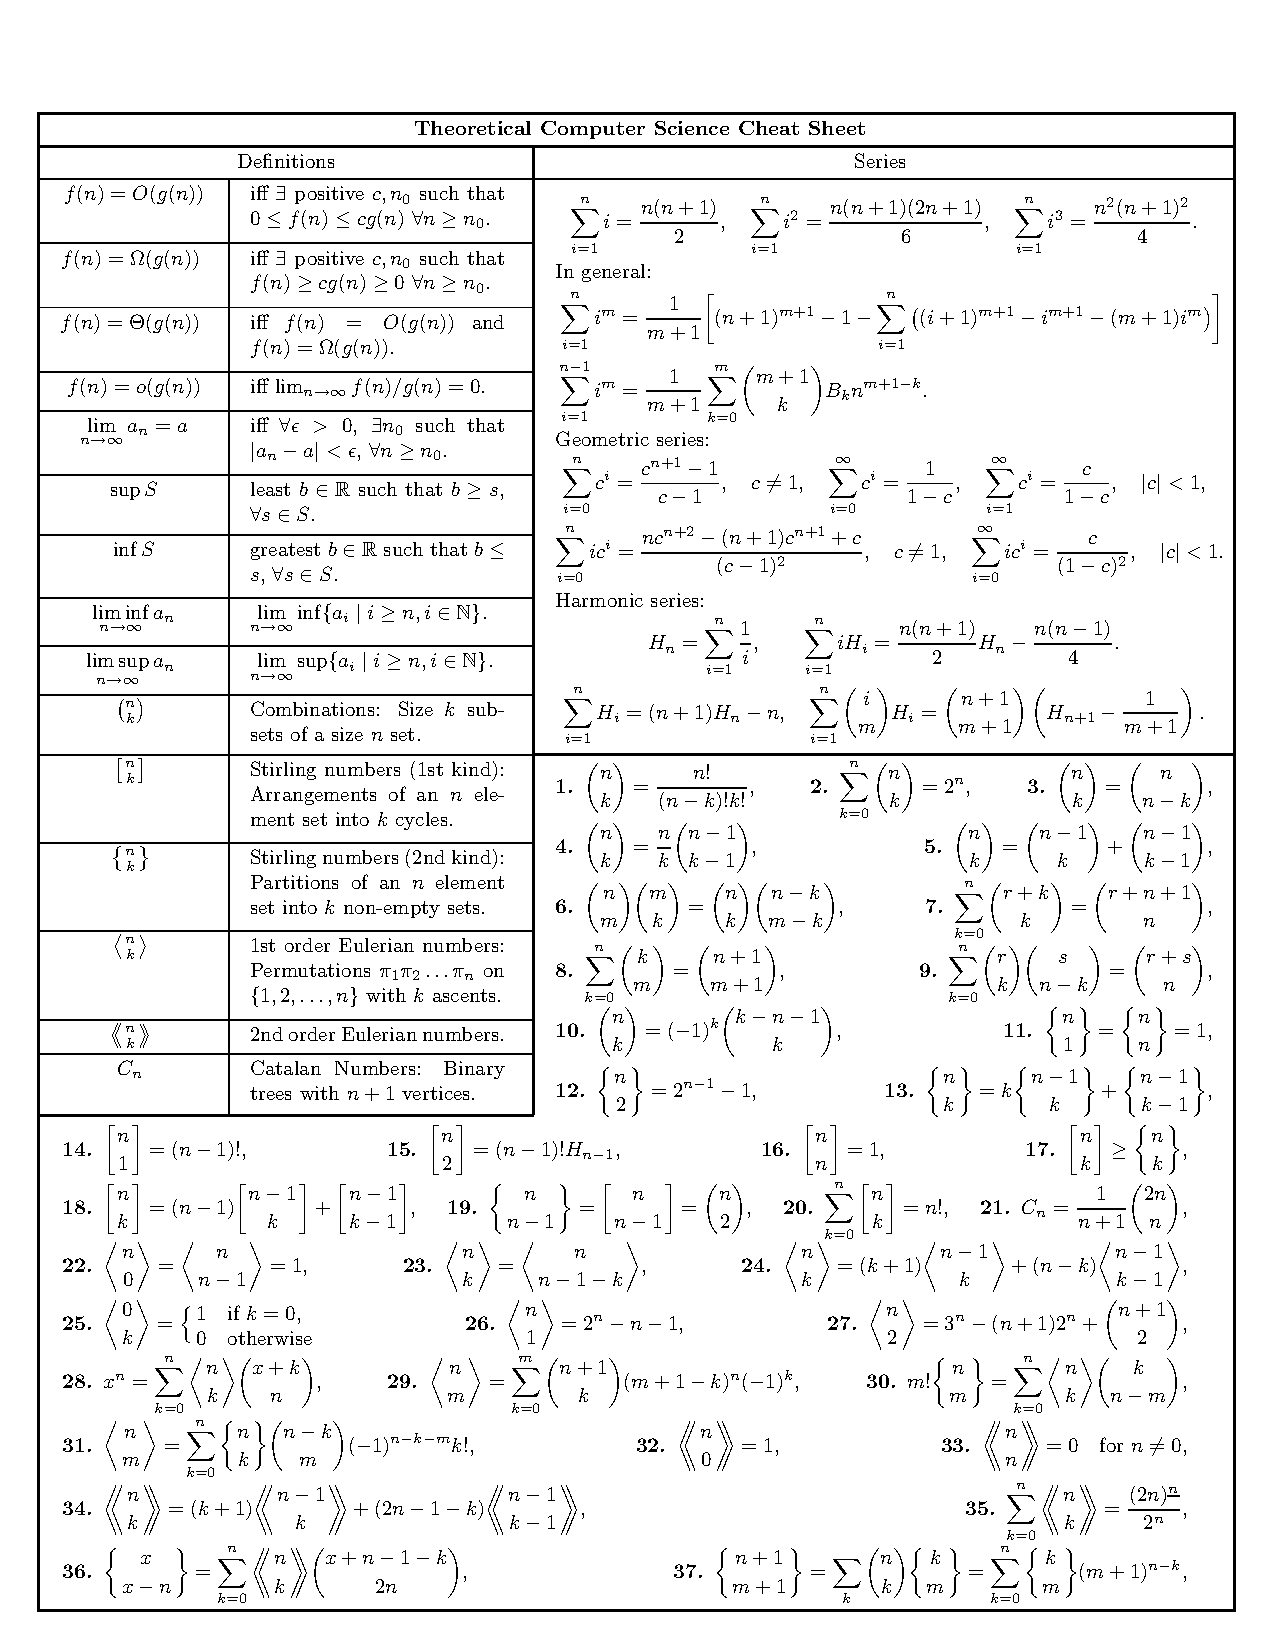
\includepdf[pages=-]{source/Appendix/cheat.pdf}
	\end{spacing}
    \section{附录}
    \subsection*{NTT素数及原根列表}
    \begin{spacing}{0.97}
\rowcolors{2}{black!25}{white}
\noindent \begin{tabular}{ccc}
\toprule
       Id & Primes & Primitive Root\\
\midrule 1 & 7340033 & 3\\
 2 & 13631489 & 15\\
 3 & 23068673 & 3\\
 4 & 26214401 & 3\\
 5 & 28311553 & 5\\
 6 & 69206017 & 5\\
 7 & 70254593 & 3\\
 8 & 81788929 & 7\\
 9 & 101711873 & 3\\
 10 & 104857601 & 3\\
 11 & 111149057 & 3\\
 12 & 113246209 & 7\\
 13 & 120586241 & 6\\
 14 & 132120577 & 5\\
 15 & 136314881 & 3\\
 16 & 138412033 & 5\\
 17 & 141557761 & 26\\
 18 & 147849217 & 5\\
 19 & 155189249 & 6\\
 20 & 158334977 & 3\\
 21 & 163577857 & 23\\
 22 & 167772161 & 3\\
 23 & 169869313 & 5\\
 24 & 185597953 & 5\\
 25 & 186646529 & 3\\
 26 & 199229441 & 3\\
 27 & 204472321 & 19\\
 28 & 211812353 & 3\\
 29 & 221249537 & 3\\
 30 & 230686721 & 6\\
 31 & 246415361 & 3\\
 32 & 249561089 & 3\\
 33 & 257949697 & 5\\
 34 & 270532609 & 22\\
 35 & 274726913 & 3\\
 36 & 290455553 & 3\\
 37 & 305135617 & 5\\
\bottomrule
\end{tabular}
\rowcolors{2}{black!25}{white}
\begin{tabular}{ccc}
\toprule
       Id & Primes & Primitive Root\\
 \midrule
 38 & 311427073 & 7\\
 39 & 330301441 & 22\\
 40 & 347078657 & 3\\
 41 & 359661569 & 3\\
 42 & 361758721 & 29\\
 43 & 377487361 & 7\\
 44 & 383778817 & 5\\
 45 & 387973121 & 6\\
 46 & 399507457 & 5\\
 47 & 409993217 & 3\\
 48 & 415236097 & 5\\
 49 & 447741953 & 3\\
 50 & 459276289 & 11\\
 51 & 463470593 & 3\\
 52 & 468713473 & 5\\
 53 & 469762049 & 3\\
 54 & 493879297 & 10\\
 55 & 531628033 & 5\\
 56 & 576716801 & 6\\
 57 & 581959681 & 11\\
 58 & 595591169 & 3\\
 59 & 597688321 & 11\\
 60 & 605028353 & 3\\
 61 & 635437057 & 11\\
 62 & 639631361 & 6\\
 63 & 645922817 & 3\\
 64 & 648019969 & 17\\
 65 & 655360001 & 3\\
 66 & 666894337 & 5\\
 67 & 683671553 & 3\\
 68 & 710934529 & 17\\
 69 & 715128833 & 3\\
 70 & 718274561 & 3\\
 71 & 740294657 & 3\\
 72 & 745537537 & 5\\
 73 & 754974721 & 11\\
 74 & 770703361 & 11\\
\bottomrule
\end{tabular}
\rowcolors{2}{black!25}{white}
\begin{tabular}{ccc}
\toprule
       Id & Primes & Primitive Root\\
 \midrule
 75 & 786432001 & 7\\
 76 & 799014913 & 13\\
 77 & 800063489 & 3\\
 78 & 802160641 & 11\\
 79 & 818937857 & 5\\
 80 & 824180737 & 5\\
 81 & 833617921 & 13\\
 82 & 850395137 & 3\\
 83 & 862978049 & 3\\
 84 & 880803841 & 26\\
 85 & 883949569 & 7\\
 86 & 897581057 & 3\\
 87 & 899678209 & 7\\
 88 & 907018241 & 3\\
 89 & 913309697 & 3\\
 90 & 918552577 & 5\\
 91 & 919601153 & 3\\
 92 & 924844033 & 5\\
 93 & 925892609 & 3\\
 94 & 935329793 & 3\\
 95 & 938475521 & 3\\
 96 & 940572673 & 7\\
 97 & 943718401 & 7\\
 98 & 950009857 & 7\\
 99 & 957349889 & 6\\
 100 & 962592769 & 7\\
 101 & 972029953 & 10\\
 102 & 975175681 & 17\\
 103 & 976224257 & 3\\
 104 & 985661441 & 3\\
 105 & 998244353 & 3\\
 106 & 1004535809 & 3\\
 107 & 1007681537 & 3\\
 108 & 1012924417 & 5\\
 109 & 1045430273 & 3\\
 110 & 1051721729 & 6\\
 111 & 1053818881 & 7\\
\bottomrule
\end{tabular}
\end{spacing}

    \end{multicols}
\end{document}
